\documentclass[a4paper,
               11pt,
               parskip=half,
               headinclude,
               titlepage=false]{scrartcl}

%%%%%%%%%%%%%%%%%%%%%%%%%%%%%%%%%%%%%%%%
\newcommand{\metaauthor}{moPsy}
\newcommand{\metatitle}{DIV User Manual}
\newcommand{\metarev}{1.1}
%%%%%%%%%%%%%%%%%%%%%%%%%%%%%%%%%%%%%%%%


\usepackage[utf8]{inputenc}

\usepackage[T1]{fontenc}        % Tries to use Postscript Type 1 Fonts for better rendering
\usepackage{lmodern}            % Provides the Latin Modern Font which offers more glyphs than the default Computer Modern
\usepackage[sfdefault]{carlito}
\usepackage[intlimits]{amsmath} % Provides all mathematical commands
\usepackage[protrusion=true,
            expansion,
            kerning=true,
            babel=true]{microtype}
\usepackage{fontawesome}

\usepackage[english]{babel}
\usepackage[english]{isodate}

\usepackage{eurosym}
\usepackage[shortlabels]{enumitem}

\usepackage{grffile}            % Allow you to include images (like graphicx). Usage: \includegraphics{path/to/file}

\usepackage[ugly]{units}        % Allows you to type units with correct spacing and font style. Usage: $\unit[100]{m}$ or $\unitfrac[100]{m}{s}$

\usepackage{xspace}             % Use \xpsace in macros to automatically insert space based on context. Usage: \newcommand{\es}{ESPResSo\xspace}
\usepackage[dvipsnames,table]{xcolor}             % Obviously colors. Usage: \color{red} Red text
\usepackage{booktabs}           % Nice rules for tables. Usage \begin{tabular}\toprule ... \midrule ... \bottomrule


%\usepackage[hang]{subfigure}  % unterteilte Abbildungen
\usepackage{setspace}          %fuer dem Zeilanabstand
\usepackage[hang,bf,footnotesize]{caption}   % bessere Bildunterschriften
\usepackage{wrapfig}

\usepackage{csquotes}


\usepackage[hyphens]{url}                % Lets you typeset urls. Usage: \url{http://...}
\usepackage[pdftex,colorlinks=true,linkcolor=black,citecolor=black,urlcolor=black]{hyperref}
\hypersetup{
  pdftitle    = {\metatitle},
  pdfsubject  = {Assembly Guide},
  pdfauthor   = {\metaauthor},
  pdfkeywords = {} ,
  pdfcreator  = {pdflatex},
  pdfproducer = {LaTeX with hyperref}
}
%%%%%%%%%%%%%%%%%%%%%%%%%%%%%%%%%%%%%%%%

\usepackage{pdfpages}

\usepackage{tabularx}


\usepackage[headsepline, footsepline]{scrlayer-scrpage}
\setlength{\headheight}{34pt} % logo height
\clearpairofpagestyles
\ohead{
\vfill%
\begin{tabular}{@{}l l@{}}

\includegraphics[height=2em]{moPsy_logo}\hspace*{-0.1cm}
\end{tabular}
}
\ihead{
\vfill%
{\huge DIV} \,v\metarev\, User Manual%
}
\ofoot{Page \thepage}
\setkomafont{pageheadfoot}{\sffamily\footnotesize}
\setkomafont{pagination}{}
\pagestyle{scrheadings}


%\usepackage{background}

%\usepackage[section]{placeins} % keep figures in their section


\definecolor{level_easy}{rgb}{0.2, 0.6, 0.1}

\definecolor{row1}{rgb}{1.0, 1.0, 1.0}
\definecolor{row2}{rgb}{0.93, 0.93, 0.99}



\begin{document}


\begin{minipage}[]{10.5cm}
\setlength{\parskip}{\medskipamount}
\section*{Thank you for choosing a 
\includegraphics[height=0.8em]{moPsy_logo} module!}

This manual provides information on installing and using the DIV module.
We hope that all questions will be answered.
If you encounter a problem or have further questions,
please do not hesitate to reach us at \href{mailto:contact@mopsy-music.de}{\texttt{contact@mopsy-music.de}}.


\vspace{1em}
\begin{center}
Enjoy your module! \quad 
\includegraphics[height=0.8em]{peace_love_music}
\end{center}

\section*{About DIV}
\emph{DIV} is a simple clock divider, similar to the \href{https://doepfer.de/a160.htm}{Doepfer A-160-1}.

This module works as a rhythm and clock divider, as expected, but also accepts audio frequencies and happily scales your waves down by several octaves (bear in mind that the output will be 50\% PWM).

The reset input can be configured for triggers from the bus gate.

\end{minipage}%
\hspace{0.5cm}
\begin{minipage}[]{4cm}
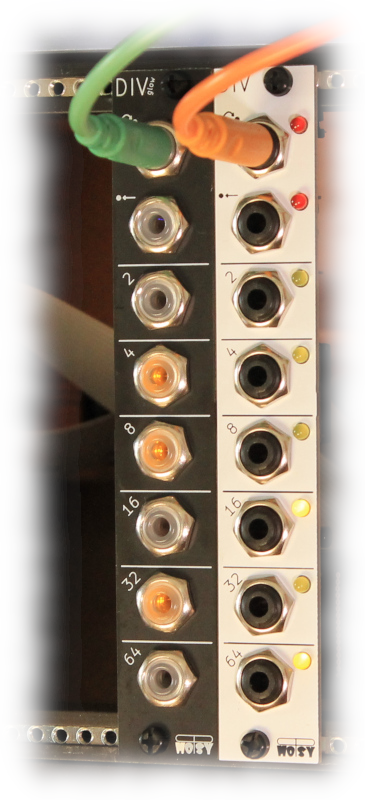
\includegraphics[width=4cm]{div-case-shot-frame}
\end{minipage}


\section*{Installation}

The DIV module will occupy \textbf{\unit[4]{HP}} in your rack with a depth of \textbf{\unit[40]{mm}}.

To \textbf{connect power} …
\begin{enumerate}
 \item Please make sure that your cabinet is \textbf{disconnected from the mains} and has no power.
 \item The module is connected with a \textbf{16-pin} (2x8) bus cable.
 \item \textbf{Check your power cable and the polarity.} The coloured ({\color{red}red}) line on the cable (pin 1) needs to be connected to the \textbf{\unit[-12]{V}} rail.
 If the module is installed in an upright orientation, the \textbf{\color{red}red stripe} needs to be \textbf{facing down}.
 \item If you plug the module backwards, it may burn out.
 Unfortunately this cannot be covered by the warranty.
\end{enumerate}

The module draws a maximum of \textbf{\unit[40]mA} from the \textbf{\unit[+12]{V}} rail.



\begin{minipage}[]{4cm}
\includegraphics[width=3.8cm, trim={0 7cm 0 0}, clip]{div-Bus-Gate-Reset}
\end{minipage}
\hspace{0.5cm}
\begin{minipage}[]{10.5cm}
\setlength{\parskip}{\medskipamount}


\section*{Setup}

Jumper \textbf{\color{red}J1} connects the module's reset to the Bus Gate, allowing for a global reset signal.

Set this jumper if you want to use the feature, otherwise we propose to just leave it on one pin of the header so that it will be available for later use.

\end{minipage}


\begin{minipage}[]{10.5cm}
\setlength{\parskip}{\medskipamount}
\section*{Frontpanel}

The \textbf{\color{red}Clock Input} advances the counter by one step on each rising edge.
Gates can also be applied, however only rising edges will have an effect.

The frequency can go well into the audible range.

If the module does not react, either the frequency is too high and an edge can no longer be detected, or the signal voltage is too low.

\vspace{1em}

On a rising edge (trigger) the \textbf{\color{red}Reset Input} will set the internal counter to zero and switch all outputs off.
The counter is blocked if this input held high (gated).

The Reset Input is mirrored on the bus side (see \emph{Setup}) with the same behavior. Both inputs can be used simultaneously.% and are OR'ed together.

\vspace{1em}

The \textbf{\color{red}Divider Output} gates are a binary representation of the internal counter. They can also be understood as divisions by the number printed next to the output.

If the internal counter reaches its capacity of 128 steps it wraps around and restarts at zero.

\end{minipage}%
\hspace{0.5cm}
\begin{minipage}[]{4cm}
\includegraphics[width=4cm]{div-frontpanel-labels}
\end{minipage}

\section*{Online Resources}

More about the module can be found …
\begin{itemize}[noitemsep]
 \item in the GitHub repository: \url{https://github.com/moPsy-project/div}
 \item on ModularGrid: \url{https://www.modulargrid.net/e/other-unknown-mopsy-div}
 \item via e-mail: \href{mailto:contact@mopsy-music.de}{\texttt{contact@mopsy-music.de}}
\end{itemize}


\end{document}
